\question{Токопрохождение в триоде при положительных и отрицательных напряжениях
  на сетке. Режимы токоперехвата и возврата электронов}

В общем случае анализ электроники триода основан на формуле для действующего
потенциала сетки:
\begin{equation}
  U_D = \sigma (U_C + D U_A),
  \label{eq21el}
\end{equation}
где \( \sigma \)~-- параметр, который носит название остроты управления и
равный приблизительно величине \( \sigma \approx 1/(1 + D) \).

Прохождение анодного тока через триод можно описать, введя представление
эквивалентного диода, то есть такого диода, у которого плоскость анода
совпадает с плоскостью сетки в триоде. В этом случае катодный ток подчиняется
классическому закону Ленгмюра:
\begin{equation}
  I_k = P(U_C + DU_A)^{3/2},
  \label{eq211}
\end{equation}
где  \( P \)~-- первеанс триода, зависящий от геометрических
размеров триод.

Введем коэффициент токопрохождения \( s = I_a/I_k \) и коэффициент
токораспределения \( k = I_a/I_c \). Оба эти коэффициента равнозначны, но чаще
используют коэффициент \( s \), зная который легко определяются величины всех
токов:
\[
  I_a = s I_k; \qquad I_c = (1 - s) I_k; \qquad \frac{s}{k} = 1 - s.
\]

Выделяют два режима работы триода:
\vspace{-.5em}
\begin{itemize}
  \itemsep -.5pt
  \item режим токоперехвата (при \( U_A > U_D \));
  \item режим возврата электронов (при \( U_A < U_D \)).
\end{itemize}

\subquestion{Режим токоперехвата}

В данном режиме ток сетки будет определяться только теми электронами, которые
будут перехватываться сеткой при их непосредственном движении от катода к аноду.

\begin{figure}[h!]
  \center
  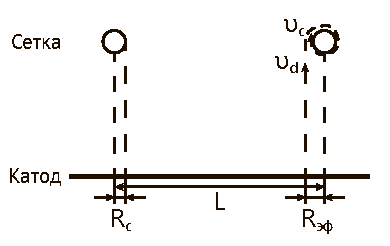
\includegraphics[width=.4\textwidth]{21_catch} \hspace{1em}
  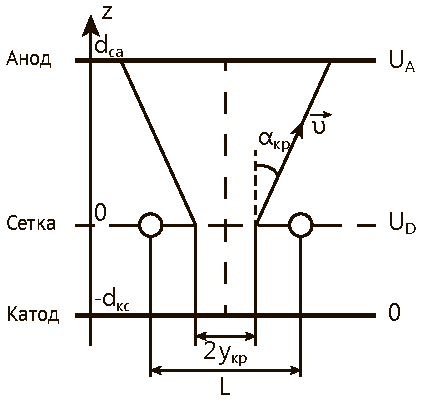
\includegraphics[width=.4\textwidth]{21_back} \\
  \vspace{-1em}\parbox{1em}{\small а)}\hspace{7.5em}\parbox{1em}{\small б)}
  \hspace{.4\textwidth}\hphantom{0} \\
  \parbox{.4\textwidth}{\caption{Режим токоперехвата} \label{pic21CC}}
  \hspace{1em}
  \parbox{.4\textwidth}{\caption{Режим возврата электронов} \label{pic21EB}}
\end{figure}

Предположим, что эмиссия электронов с катода равномерна и прямолинейна.
Тогда коэффициент токопрохождения будет определяться отношением площади катода, не
находящейся под поверхностью сетки, к полной площади катода (рис.~\pic{21CC}а):
\begin{equation}
  s_0 = \frac{L_\text{не под сеткой}}{L} = \frac{L - 2 R_c}{L} =
    1 - \frac{2 R_c}{L}.
  \label{eq21s0}
\end{equation}

В зависимости от знака напряжения на сетке \( U_C \) может наблюдаться
два случая: при \( U_C < 0 \) коэффициент токопрохождения \( s \) будет больше
\( s_0 \), а при \( U_C > 0 \)~-- меньше \( s_0 \).

Рассмотрим второй случай.

Пускай электрон вылетает на некотором расстоянии \( R_\text{эф} \) от центра
элемента сетки (рис.~\pic{21CC}б).

По закону сохранения момента импульса (при нулевой начальной скорости
электрона):
\[
  m v_d R_\text{эф} = m v_c R_c.
\]

Выразим скорости из закона сохранения энергии:
\[
  \frac{m v_d^2}{2} = e U_D, \quad \frac{m v_c^2}{2} = e U_C; \quad \Rightarrow
    \quad v_d = \sqrt{\frac{2 e}{m} U_D}, \quad v_c = \sqrt{\frac{2 e}{m} U_C}.
\]

Тогда \( R_\text{эф} = R_c \cdot \sqrt{U_C / U_D} \). Подставляя в \eqref{eq21s0}
\( R_\text{эф} \) вместо \( R_c \), получим
\begin{equation}
  s = 1 - \frac{2 R_\text{эф}}{L} = 1 - \frac{2 R_c}{L} \sqrt{\frac{U_C}{U_D}}.
  \label{eq21dntt}
\end{equation}

Из формулы~\eqref{eq21el} следует, что \( U_C = U_D / \sigma - D U_A \); подставим
в~\eqref{eq21dntt}:
\[
  s = 1 - \frac{2 R_c}{L} \sqrt{\frac{U_D}{\sigma U_D} - \frac{D U_A}{U_D}} =
    1 - \frac{2 R_c}{L} \sqrt{\frac{1}{\sigma} - D \frac{U_A}{U_D}}.
\]

\subquestion{Режим возврата электронов}

Режим возврата электронов возникает, когда между сеткой и анодом действует
тормозящее поле, возвращающее часть электронов обратно к сетке.

Представим траекторию электрона в виде ломаной кривой (рис.~\pic{21EB}).

У крайнего электрона перпендикулярная аноду составляющая скорости равна нулю,
пройдя область сетки он вылетает под углом \( \alpha_\text{кр} \):
\[
  e (U_D - U_A) = \frac{m (v_d \cos\alpha_\text{кр})^2}{2}.
\]
Так как \( e U_D = m v_d^2 / 2 \), то
\( \sin\alpha_\text{кр} = \sqrt{U_A / U_D} \).

Анода будут достигать те электроны, которые вылетают под углом
\( \alpha < \alpha_\text{кр} \).

Действие сетки на электрон аналогично действию рассеивающей линзы-диафрагмы,
оптическая сила которой:
\[
  \frac{1}{f} = \frac{1}{4 \sqrt{U_0}} \int\lii \frac{U_0''}{\sqrt{U_0}}\,dz.
\]

Считая, что \( U_0'' \ne 0 \) только при \( z = 0 \), то \( U_0 = U_D \) и
\[
  \frac{1}{f} = \frac{1}{4 U_D} \int\lii U_0''\,dz = \frac{1}{4 U_D} \left(
    \frac{U_A - U_D}{d_\text{са}} - \frac{U_D}{d_\text{кс}} \right).
\]

Тогда фокусное расстояние:
\[
  f = 4 U_D \frac{d_\text{са} d_\text{кс}}{d_\text{кс} (U_A - U_D) -
    d_\text{са} U_D} = 4 U_D \frac{d_\text{са} d_\text{кс}}
    {d_\text{кс} U_A - d_\text{ка} U_D},
\]
где \( d_\text{ка} = d_\text{кс} + d_\text{са} \)~-- расстояние от катода до
анода.

Так как \( d_\text{кс} \ll d_\text{ка} \), то
\[
  f \approx -4 U_D \frac{d_\text{са} d_\text{кс}}{d_\text{ка} U_D} = 
    -4 \frac{d_\text{са} d_\text{кс}}{d_\text{ка}}.
\]

Тогда \( \tg\alpha_\text{кр} = y_\text{кр} / f \), а так как
\( \alpha_\text{кр} \) мало, то \( \tg\alpha_\text{кр} \sim
\sin\alpha_\text{кр} \).

Получаем, что
\[
  y_\text{кр} = f \sin\alpha_\text{кр} = f \sqrt{\frac{U_A}{U_D}} =
    4 \frac{d_\text{са} d_\text{кс}}{d_\text{ка}} \sqrt{\frac{U_A}{U_D}}.
\]

Таким образом, коэффициент токопрохождения, аналогично \eqref{eq21s0}:
\[
  s = \frac{I_a}{I_k} = \frac{2 y_\text{кр}}{L} =
    4 \frac{d_\text{са} d_\text{кс}}{d_\text{ка} L} \sqrt{\frac{U_A}{U_D}}.
\]

На рисунке \pic{21dis} приведена типичная кривая токораспределения (без учета
начальных скоростей электронов и полей пространственного заряда).

\begin{figure}[h!]
  \center
  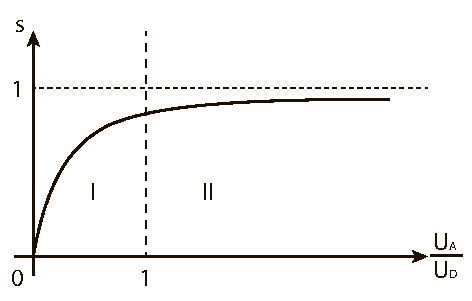
\includegraphics[width=.5\textwidth]{21_distribution}
  \caption{Кривая токораспределения в плоском триоде\\
  I~-- область возврата электронов; II~-- область токоперехвата}
  \label{pic21dis}
\end{figure}